\chapter[SCP-008 丧尸病毒]{
	SCP-008 Zombie Plague\\
	SCP-008 丧尸病毒\footref{foot:fix}
}

\label{chap:SCP-008}

\begin{scpbox}[center upper]

\GG{\tred{\bb{由于监督委员会的命令}}}

\Gg{该文档被分类为4级}

\GG{\tred{\bb{==访问需4级权限 ==}}}

\end{scpbox}

\cl{

\tred{- 请输入安保证号 -}

\tred{- 安保权限充足,提取文件…}

}

\begin{figure}[H]
	\centering
	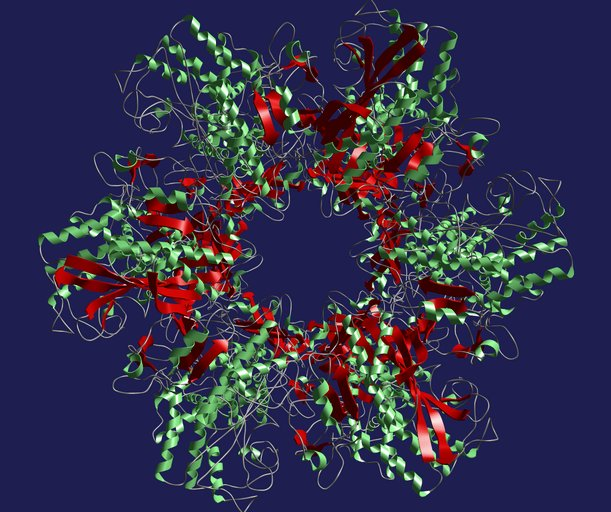
\includegraphics[width=0.5\linewidth]{images/SCP.008.jpg}
	\caption*{显示出SCP-008的三级结构的色带图。\\主要氨基酸序列信息已被删节。}
\end{figure}

\bb{项目编号:}SCP-008

\bb{项目等级:}Euclid

\bb{特殊收容措施:}SCP-008样本被视为 V级 极端生物危害且适用于所有相关协议。焚烧和辐射措施将被用于操作员或外部频道在任何给定的8小时内保持零通讯、电源故障、可能会导致设施被拆除的政治或军事行动的情况下。

离开操作设施的员工将被隔离四个月。如果违反,将实施焚烧和辐射措施。这将是应用于所有不作撤离准备程序的G2站点的政策。

\bb{描述:}SCP-008是一种复杂的朊病毒,所有已知的G2站点都储存有它的样本。关于SCP-008的研究是高度机密,目的主要在于预防的研究,这将使合成SCP-008在遥远的将来成为可能。SCP-008朊病毒的性状包括:

\begin{itemize}
\item 传染性100\%。
\item 致死性100\%。
\item 通过裸露的黏膜和所有体液进行传播。
\item 不能在空气和水中传播。
\end{itemize}

暴露于SCP-008后不超过三小时的感染症状包括:

\begin{itemize}
\item 出现类似流感的症状,发高烧,后期阶段重度痴呆。
\item 在最初症状出现并经过12小时明显的痴呆症后,昏迷约20小时。昏迷将被视为发病死亡。
\item 一段时期内出现散发性的细胞坏死,其中具有某些类似于坏疽的症状。尚存的组织承担原有的功能,具有高度弹性。
\item 血红细胞大大增加储氧能力,使血流减缓、肌肉的耐力和力量增加。
\item 总器官功能衰竭几小时后,神经和肌肉系统仍不受影响。
代谢会下降到极低的水平,使感染者能在无营养条件的情况下存活超过十年。
\item 高度的血液粘稠度使感染者在受到枪击、穿刺和砍伤的情况下产生可忽略不计的出血量。
\item 条件反射的行为,运动神经的控制能力,和本能的行为机制被破坏,认知能力严重减弱且不稳定。动物实验中出现过多的脑细胞坏死并处于非活动状态。
\item 受体能适应其受损的神经系统,但仅限于基本的身体活动,包括站起,双腿保持平衡,行走,咬,抢夺,和爬行。感染者会尽量朝向能与活体人类联系的景象、声音、气味的方向移动。如果感染者与活的人类产生身体接触,会试图摄入目标。
\item 压制完全感染者需要予以造成极强的颅外伤。
\end{itemize}

强有力的证据表明SCP-008不是在地球上自然形成的,因为复杂度类似的变异体无法存在于生态系统中。1959年,苏联发现SCP-008后,与苏联谈判达成了一次简短的合作以建立G2站点并抹消SCP-008。合作结束后,SCP-008在俄罗斯的保管状况是未知的。

\bb{附录008-1:}SCP-500被发现即使在该病的晚期阶段仍能彻底治愈SCP-008。
